% Introduction

\chapter{Introduction} % Main chapter title
\label{Introduction} % For referencing the chapter elsewhere, use \ref{Chapter1} 

\hyphenation{area}
\hyphenation{areas}

\startcontents[chapters]
\Mprintcontents

%----------------------------------------------------------------------------------------

% Define some commands to keep the formatting separated from the content 

%----------------------------------------------------------------------------------------


\section{Analysis of forested areas}
Forests are a core component of planet's life. They are defined as large area dominated by trees. Hundreds of other definitions of forest may be used all other the world, incorporating factors such as tree density, tree height, land use, legal standing and ecological function \citep{schuck2002compilation,achard2009vital}.

Forest are commonly defined as land with tree crown cover (or equivalent stocking level) of more than 10 percent and area of more than 0.5 hectares (ha). The trees should be able to reach a minimum height of 5 meters at maturity in situ. They may consist either of closed forest formations where trees of various storeys and undergrowth cover a high proportion of the ground; or open forest formations with a continuous vegetation cover in which tree crown cover exceeds 10 percent. Young natural stands and all plantations established for forestry purposes which have yet to reach a crown density of 10 percent or tree height of 5 m are included under forest, as are areas normally forming part of the forest area which are temporarily unstocked as a result of human intervention or natural causes but which are expected to revert to forest.

\begin{figure}[htbp]
\begin{center}
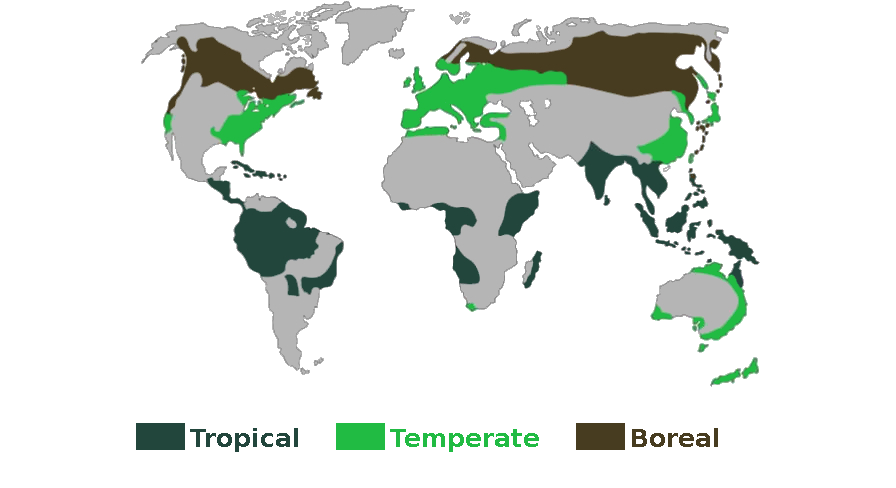
\includegraphics[width=\textwidth]{Figures/forest_in_world.png}
\caption{Forest repartition and categorization in the world.}
\label{fig:forest_in_world}
% source : http://dyntatrishana.blogspot.fr/2015/11/about-value-of-forests.html
\end{center}
\end{figure}

Forests are the dominant terrestrial ecosystem of Earth, and are distributed across the globe \citep{pan2013structure}. They cover about four billion hectares, or approximately 30\% of the world's land area (see Figure~\ref{fig:forest_in_world}). Forests at different latitudes and elevations form distinctly different ecozones: boreal forests near the poles, tropical forests near the Equator and temperate forests at mid-latitudes (see Figure~\ref{fig:forest_in_world}). Higher elevation areas tend to support forests similar to those at higher latitudes, and the amount of precipitation also affects forest composition. Since these ecozones are very different, the study at a fine level (e.g. species composition) of forested areas must be restricted to a single ecozone at a time.

Human society and forests influence each other in both positive and negative ways \citep{vogt2006global}. Human activities, including harvesting forest resources, can negatively affect forest ecosystems. Forests have 3 main contributions to human: ecosystem services, tourist attraction and harvesting.

\textbf{\underline{Ecosystem services.}}\\
Forests provide ecosystem services. Indeed, Forests account for 75\% of the gross primary productivity of the Earth's biosphere, and contain 80\% of the Earth's plant biomass \citep{pan2013structure}. They also hold about 90\% of terrestrial biodiversity \citep{brooks2006global, wasiq2004sustaining}. Forests are also beneficial for the environment; they capt and store the CO$_{2}$ \citep{fahey2010forest} (see Figure~\ref{fig:carbon_cycle}). About 45\% of the total global carbon is held by forests. They also filter dust and microbial pollution of the air \citep{smith2012air}. Finally, they also play an important role in hydrological regulation and water purification \citep{lempriere2008importance} (see Figure~\ref{fig:carbon_cycle}).

\begin{figure}[htbp]
\begin{center}
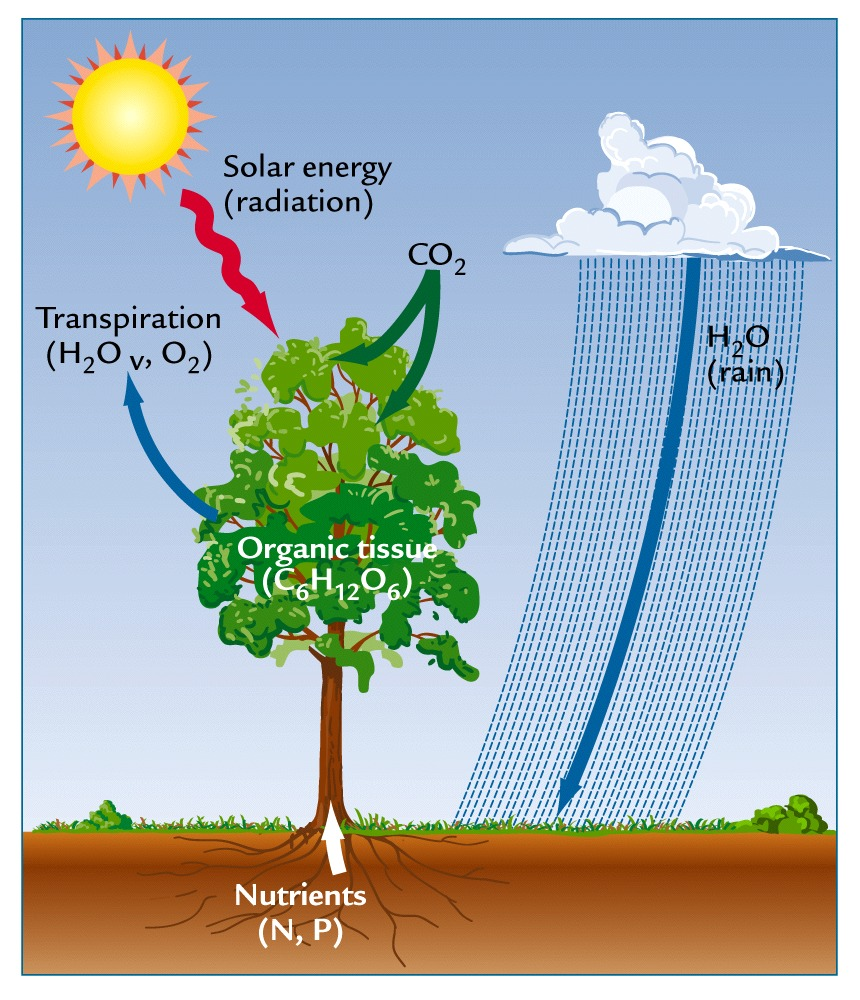
\includegraphics[width=0.5\textwidth]{Figures/carbon_cycle}
\caption{Carbon cycle: a process of CO$_{2}$ storage, water and air purification.}
% source :http://www.atmosedu.com/Geol390/Life/CarbonCycleShort.html
\label{fig:carbon_cycle}
\end{center}
\end{figure}

\textbf{\underline{Tourist attraction.}}\\
Forests serve as tourist attractions. In France, there are hundred of long distance footpaths ($\sim$ 60000km) through forests. Other activities such as rock climbing, mountain bike or adventure parks are mostly practiced in forests.

\textbf{\underline{Harvesting.}} \\
Wood from trees displays many uses. It has been widely used for fuel \citep{sterrett1994alternative}. In this case, hardwood is preferred over softwood because it creates less smoke and burns longer. 
Wood is still an important construction material \citep{ramage2017wood}: Elm was used for the construction of wood boats. In Europe, oak is still the preferred variety for all wood constructions, including beams, walls, doors, and floors. A wider variety of woods is also used such as poplar, small-knotted pine, and Douglas fir.
Wood is also needed in the paper industry since wood fibers are an important component of most papers. Eventually, wood is also extensively used for furniture or for making tools or music instruments. \\

The evolution of forests need to be monitored in order to exploit efficiently the forest resources in a sustainable way (Paris Agreement). For example, France is a great wood importer ($\sim$ 25 millions of m$^{3}$ per year), while the french forest is the third in Europe in term of volume. It is therefore needed to better manage and exploit the french wood stocks.

In order to evaluate the forest resources, a precise mapping of forests is needed.
Forests are complex structures \citep{pommerening2002approaches}, for which information is needed for management, exploitation and more generally for public and private policies. Such information can be the tree species or the tree maturity of the forest. There are two ways to extract such information from forest; \textbf{field inventory} or \textbf{remote sensing}. The field inventories are very expensive to set up and are also not adapted for a national mapping, but is more adapted for statistics. Remote sensing is a more relevant way in order to obtain such information since it allows to extract them at a large scale. \\

In order to meet these needs, two synergistic products could be produced: a statistical inventory or a forest mapping.

\section{Remote sensing for forested areas}

The analysis of forested areas from a remote sensing point of view can be performed at three different levels: pixel, object (mainly trees) or stand. In statistical national forest inventory (NFI), an automated and accurate tree segmentation is needed in order to extract tree level features (basal area, dominant tree height, etc., \citep{means2000predicting,Malatamo}). However, the tree level is not the only reliable level of analysis for forest studies at a national scale but could be employed for a local study. When a joint mapping and statistical reasoning is required (e.g., land-cover (LC) mapping and forest inventory \citep{tomppo2008combining}), forest stands remain the prevailing scale of analysis \citep{means2000predicting,White2016CJRS}. A stand can be defined in many different ways in terms of homogeneity: tree specie, age, height, maturity, and its definition varies according to the countries. \\

From a remote sensing point of view, the delineation of the stands is a segmentation problem. Forest stands are preferred, since they allow to extract reliable and statistically meaningful features and to provide an input for multi-source statistical inventory. For land-cover mapping, this is highly helpful for forest database updating \citep{Kim09}, whether the labels of interest are \textit{vegetated areas} {(e.g., \textit{deciduous/evergreen/mixed/non-forested)}}, or, even more precisely, the tree species. To obtain such information, most of the time in national forestry inventory institutes, for reliability purposes, each area is manually interpreted by human operators with very high resolution (VHR) geospatial images focusing on the infra-red channel \citep{Malatamo}. This work is extremely time consuming and subjective \citep{Wulder2008}. Furthermore, in many countries, the wide variety of tree species (e.g., $>$20) significantly complicates the problem. This is all the more true than photo-interpretation may not always be sufficient and even in case of few species (3-5), automatic classification techniques are not effective enough. The design of an automatic procedure based on remote sensing data would fasten and ease such process. Additionally, the standard manual delineation procedure only takes into account the species, and few characteristics (alternatively height, age, stem density or crown closure). Instead, an automatic method could offer more flexibility being not limited to a visual analysis and using characteristics extracted from complementary data sources and not only CIR ortho-images. \\

The use of remote sensing data for the automatic analysis of forests has been growing in the last 15 years, especially with the synergistic use of airborne laser scanning (ALS) and optical VHR imagery (multispectral imagery and hyperspectral imagery) \citep{torabzadeh2014fusion,White2016CJRS}. Several countries have already integrated such sources in their operational pipeline for forest management and characterization. They appear to be both well adapted and complementary inputs for stand segmentation \citep{dalponte2012tree,dalponte2015delineation,7500049}. Furthermore, they can be employed for forest management \citep{tokola2015remote, wulder2008role, patenaude2005synthesis}. ALS provides a joint direct access to the vertical distribution of the trees and to the ground underneath \citep{holmgren2004prediction}. Hyperspectral and multispectral optical images are particularly relevant for tree species classification: spectral and textural information from VHR  images can allow a fine discrimination of many species. Multispectral images are often preferred due to their higher availability, and higher spatial resolution. Multispectral images can be acquired from airplanes or satellites. Spaceborne sensors allow to capture large areas with a high temporal rate but suffer from a lower spatial resolution, even if the gap decreases every year (see Table~\ref{table:spatial_satellites}). For a better spatial resolution, airborne multispectral images are preferred since they allow to extract texture features that are very relevant for tree species classification \citep{franklin2000incorporating}. The airborne linear lidar has been widely used for remote sensing tasks \citep{lim2003lidar, shan2008topographic, vosselman2010airborne}. Lidar has been successfully employed for many forest applications \citep{ferraz2016lidar}. The new Geiger mode lidar \citep{ullrich2016linear} and single photon lidar \citep{viterbini1987single} is also very promising, allowing a significantly higher point density with different angles at a higher altitude and could have an important impact of especially on the studies of forested areas \citep{jakubowski2013tradeoffs, strunk2012effects}. \\

Synthetic Aperture Radar (SAR) is widely employed the the evaluation of biomass, especially in forested environment \citep{le1992relating, beaudoin1994retrieval}. With its ability to penetrate the vegetation, SAR in P-band (0.3-1$\:$GHz) allows to estimate efficiently the aboveground biomass. Thus, SAR can be employed in order to extract relevant information of forests but not for their mapping. 

\begin{sidewaystable}
\begin{center}
\begin{tabular}{l|c|c|c|c|c|c|c|c}
& \textbf{SPOT 6,7} & \textbf{Ikonos} & \textbf{Quickbird} & \textbf{Pléiades} & \textbf{RapidEye} & \textbf{Sentinel 2} & \textbf{Landsat 7} & \textbf{Worldview 3}\\
\hline
Swath & 60$\:$km & 11$\:$km & 16.5$\:$km & 20$\:$km & 77$\:$km & 290$\:$km & 185$\:$km & 13.1$\:$\\
Revisit time & 2$\:$d & 2$\:$d & 1-3.5$\:$d & 1$\:$d & 5.5$\:$d & 5$\:$d & 16$\:$d & <1$\:$d\\
Resolution & 6$\:$m & 4$\:$m & 2.44-2.88$\:$m & 2.8$\:$m & 6.5$\:$m & 10$\:$m & 30$\:$m & 1.24$\:$m\\
Number of bands & 4 & 4 & 4 & 4 & 5 & 13 & 8 & 28\\
Main spectral bands (nm) & & & & & & & &\\
Blue & 455-520 & 450-530 & 450-520 & 430-550 & 440-510 & 460-520 & 450-520 & 450-510\\ 
Green & 530-600 & 520-610 & 520-600 & 500-620 & 520-590 & 545-575 & 520-600 & 510-580\\
Red & 620-690 & 640-720 & 630-690 & 590-710 & 630-685 & 650-680 & 630-690 & 630-690\\
NIR & 760-890 & 760-880 & 760-900 & 740-940 & 760-850 & 785-900 & 760-900 & 770-895\\
\end{tabular}
\end{center}
\caption{Principal multispectral spatial optical sensors.}
\label{table:spatial_satellites}
\end{sidewaystable}

\section{Context of the thesis}
In France, the study of forests is two fold. They need to be mapped and inventoried. The forest inventory allows to obtain an estimation of the wood stock and the forestation rate at a national scale (see Figures~\ref{fig:wood_volume}~\&~\ref{fig:forestation}). Statistics such as volume per hectare, deciduous volume or conifer volume can then be derived. The inventory is performed through field inventory and extrapolated using the forest mapping. Thus, the mapping of forest is very important in order to derive accurate statistics.	

Forest mapping is traditionally provided through a national forest LC database (see Figure~\ref{fig:FLC}). It is manually interpreted by human operators using VHR colored infra-red (CIR) ortho-images. It assigns a vegetation type to each mapped beach of more than 5000$\:$m$^{2}$. The nomenclature is composed of 32 classes based on hierarchical criteria such as pure stands of the main tree species of the French forest. The forest LC should be updated in a 10 years cycle.

\begin{figure}[htbp]
\begin{center}
\begin{tikzpicture}
\def\rb{3}
\def\re{4}
\newcommand{\col}{red}

\newcommand{\arccam}[3]
{
\def\rb{3}
\def\re{4}
\def\ab{#1}
\def\ae{#2}
\def\co{#3}
\draw[fill=\co,draw=none] (0,0) -- (\ab:\re) arc (\ab:\ae:\re) -- (0,0);
}

\definecolor{perso}{RGB}{22, 184, 78}
\renewcommand{\col}{perso}


\pgfmathsetmacro\abb{0}
\pgfmathsetmacro\aee{0.12*360}
\arccam{\abb+0.5}{\aee-0.5}{\col}
\pgfmathsetmacro\amid{(\abb+\aee)/2}
\pgfmathsetmacro\px{3.5*cos(\amid)}
\pgfmathsetmacro\py{3.5*sin(\amid)}
\node[color=white] at (\px,\py) {12\%};
\pgfmathsetmacro\px{5*cos(\amid)}
\pgfmathsetmacro\py{5*sin(\amid)}
\node[color=\col,text width=50, text centered] at (\px,\py) {European oak};


\definecolor{perso}{RGB}{20, 148, 20}
\pgfmathsetmacro\abb{\aee}
\pgfmathsetmacro\aee{\abb+0.11*360}
\arccam{\abb+0.5}{\aee-0.5}{\col}
\pgfmathsetmacro\amid{(\abb+\aee)/2}
\pgfmathsetmacro\px{3.5*cos(\amid)}
\pgfmathsetmacro\py{3.5*sin(\amid)}
\node[color=white] at (\px,\py) {11\%};
\pgfmathsetmacro\px{4.0*cos(\amid)}
\pgfmathsetmacro\py{4.0*sin(\amid)}
\node[color=\col,text width=75, text centered, anchor=south west] at (\px,\py) {Sessile oak};


\definecolor{perso}{RGB}{86, 130, 3}
\pgfmathsetmacro\abb{\aee}
\pgfmathsetmacro\aee{\abb+0.10*360}
\arccam{\abb+0.5}{\aee-0.5}{\col}
\pgfmathsetmacro\amid{(\abb+\aee)/2}
\pgfmathsetmacro\px{3.5*cos(\amid)}
\pgfmathsetmacro\py{3.5*sin(\amid)}
\node[color=white] at (\px,\py) {10\%};
\pgfmathsetmacro\px{4.5*cos(\amid)}
\pgfmathsetmacro\py{4.5*sin(\amid)}
\node[color=\col,text width=50, text centered] at (\px,\py) {Beech};


\definecolor{perso}{RGB}{24, 57, 30}
\pgfmathsetmacro\abb{\aee}
\pgfmathsetmacro\aee{\abb+0.05*360}
\arccam{\abb+0.5}{\aee-0.5}{\col}
\pgfmathsetmacro\amid{(\abb+\aee)/2}
\pgfmathsetmacro\px{3.5*cos(\amid)}
\pgfmathsetmacro\py{3.5*sin(\amid)}
\node[color=white] at (\px,\py) {5\%};
\pgfmathsetmacro\px{4.0*cos(\amid)}
\pgfmathsetmacro\py{4.0*sin(\amid)}
\node[color=\col,text width=50, text centered, anchor=south east] at (\px,\py) {Chestnut};


\definecolor{perso}{RGB}{89, 102, 67}
\pgfmathsetmacro\abb{\aee}
\pgfmathsetmacro\aee{\abb+0.04*360}
\arccam{\abb+0.5}{\aee-0.5}{\col}
\pgfmathsetmacro\amid{(\abb+\aee)/2}
\pgfmathsetmacro\px{3.5*cos(\amid)}
\pgfmathsetmacro\py{3.5*sin(\amid)}
\node[color=white] at (\px,\py) {4\%};
\pgfmathsetmacro\px{4.1*cos(\amid)}
\pgfmathsetmacro\py{4.1*sin(\amid)}
\node[color=\col,text width=50, text centered,anchor=south east] at (\px,\py) {Hornbeam};


\definecolor{perso}{RGB}{1, 121, 111}
\pgfmathsetmacro\abb{\aee}
\pgfmathsetmacro\aee{\abb+0.04*360}
\arccam{\abb+0.5}{\aee-0.5}{\col}
\pgfmathsetmacro\amid{(\abb+\aee)/2}
\pgfmathsetmacro\px{3.5*cos(\amid)}
\pgfmathsetmacro\py{3.5*sin(\amid)}
\node[color=white] at (\px,\py) {4\%};
\pgfmathsetmacro\px{4.0*cos(\amid)}
\pgfmathsetmacro\py{4.0*sin(\amid)}
\node[color=\col,text width=85, text centered,anchor=south east] at (\px,\py) {Pubescent oak};


\definecolor{perso}{RGB}{88, 111, 45}
\pgfmathsetmacro\abb{\aee}
\pgfmathsetmacro\aee{\abb+0.04*360}
\arccam{\abb+0.5}{\aee-0.5}{\col}
\pgfmathsetmacro\amid{(\abb+\aee)/2}
\pgfmathsetmacro\px{3.5*cos(\amid)}
\pgfmathsetmacro\py{3.5*sin(\amid)}
\node[color=white] at (\px,\py) {4\%};
\pgfmathsetmacro\px{5*cos(\amid)}
\pgfmathsetmacro\py{5*sin(\amid)}
\node[color=\col,text width=50, text centered] at (\px,\py) {Ash};


\definecolor{perso}{RGB}{64, 130, 109}
\pgfmathsetmacro\abb{\aee}
\pgfmathsetmacro\aee{\abb+0.14*360}
\arccam{\abb+0.5}{\aee-0.5}{\col}
\pgfmathsetmacro\amid{(\abb+\aee)/2}
\pgfmathsetmacro\px{3.5*cos(\amid)}
\pgfmathsetmacro\py{3.5*sin(\amid)}
\node[color=white] at (\px,\py) {14\%};
\pgfmathsetmacro\px{5*cos(\amid)}
\pgfmathsetmacro\py{5*sin(\amid)}
\node[color=\col,text width=70, text centered] at (\px,\py) {Other hardwood};

%%%%%%%%%%%%%%%%%%%%%%%%%%%%%%%%%%%%%%%%%%%%%%%%%%

\definecolor{perso}{RGB}{136, 77, 167}
\pgfmathsetmacro\abb{\aee}
\pgfmathsetmacro\aee{\abb+0.08*360}
\arccam{\abb+0.5}{\aee-0.5}{\col}
\pgfmathsetmacro\amid{(\abb+\aee)/2}
\pgfmathsetmacro\px{3.5*cos(\amid)}
\pgfmathsetmacro\py{3.5*sin(\amid)}
\node[color=white] at (\px,\py) {8\%};
\pgfmathsetmacro\px{4.0*cos(\amid)}
\pgfmathsetmacro\py{4.0*sin(\amid)}
\node[color=\col,text width=85, text centered, anchor=north east] at (\px,\py) {Pectinated fir};


\definecolor{perso}{RGB}{102, 0, 255}
\pgfmathsetmacro\abb{\aee}
\pgfmathsetmacro\aee{\abb+0.08*360}
\arccam{\abb+0.5}{\aee-0.5}{\col}
\pgfmathsetmacro\amid{(\abb+\aee)/2}
\pgfmathsetmacro\px{3.5*cos(\amid)}
\pgfmathsetmacro\py{3.5*sin(\amid)}
\node[color=white] at (\px,\py) {8\%};
\pgfmathsetmacro\px{4.5*cos(\amid)}
\pgfmathsetmacro\py{4.5*sin(\amid)}
\node[color=\col,text width=50, text centered] at (\px,\py) {Spruce};


\definecolor{perso}{RGB}{112, 41, 99}
\pgfmathsetmacro\abb{\aee}
\pgfmathsetmacro\aee{\abb+0.06*360}
\arccam{\abb+0.5}{\aee-0.5}{\col}
\pgfmathsetmacro\amid{(\abb+\aee)/2}
\pgfmathsetmacro\px{3.5*cos(\amid)}
\pgfmathsetmacro\py{3.5*sin(\amid)}
\node[color=white] at (\px,\py) {6\%};
\pgfmathsetmacro\px{4.0*cos(\amid)}
\pgfmathsetmacro\py{4.0*sin(\amid)}
\node[color=\col,text width=75, text centered, anchor=north west] at (\px,\py) {Scots pine};


\definecolor{perso}{RGB}{46, 0, 108}
\pgfmathsetmacro\abb{\aee}
\pgfmathsetmacro\aee{\abb+0.05*360}
\arccam{\abb+0.5}{\aee-0.5}{\col}
\pgfmathsetmacro\amid{(\abb+\aee)/2}
\pgfmathsetmacro\px{3.5*cos(\amid)}
\pgfmathsetmacro\py{3.5*sin(\amid)}
\node[color=white] at (\px,\py) {5\%};
\pgfmathsetmacro\px{4.0*cos(\amid)}
\pgfmathsetmacro\py{4.0*sin(\amid)}
\node[color=\col,text width=85, text centered, anchor=north west] at (\px,\py) {Maritime pine};


\definecolor{perso}{RGB}{75, 0, 130}
\pgfmathsetmacro\abb{\aee}
\pgfmathsetmacro\aee{\abb+0.04*360}
\arccam{\abb+0.5}{\aee-0.5}{\col}
\pgfmathsetmacro\amid{(\abb+\aee)/2}
\pgfmathsetmacro\px{3.5*cos(\amid)}
\pgfmathsetmacro\py{3.5*sin(\amid)}
\node[color=white] at (\px,\py) {4\%};
\pgfmathsetmacro\px{4.0*cos(\amid)}
\pgfmathsetmacro\py{4.0*sin(\amid)}
\node[color=\col,text width=75, text centered, anchor=north west] at (\px,\py) {Douglas fir};


\definecolor{perso}{RGB}{108, 2, 119}
\pgfmathsetmacro\abb{\aee}
\pgfmathsetmacro\aee{\abb+0.05*360}
\arccam{\abb+0.5}{\aee-0.5}{\col}
\pgfmathsetmacro\amid{(\abb+\aee)/2}
\pgfmathsetmacro\px{3.5*cos(\amid)}
\pgfmathsetmacro\py{3.5*sin(\amid)}
\node[color=white] at (\px,\py) {5\%};
\pgfmathsetmacro\px{5*cos(\amid)}
\pgfmathsetmacro\py{5*sin(\amid)}
\node[color=\col,text width=50, text centered] at (\px,\py) {Other conifers};


\draw[fill=white,draw=none] (0,0) circle (\rb);

\definecolor{perso}{RGB}{108, 2, 119}
\node[color=\col] at (0,-1) {\textbf{Conifers: }};
\node[color=\col] at (0,-1.5) {\textbf{920 millions m$^{2}$}};

\definecolor{perso}{RGB}{86, 130, 3}
\node[color=\col] at (0,1.5) {\textbf{Hardwood: }};
\node[color=\col] at (0,1) {\textbf{1647 millions m$^{2}$}};

\end{tikzpicture}
\caption{Distribution wood volume per species.}
\label{fig:wood_volume}
\end{center}
\end{figure}

\begin{figure}
\begin{center}
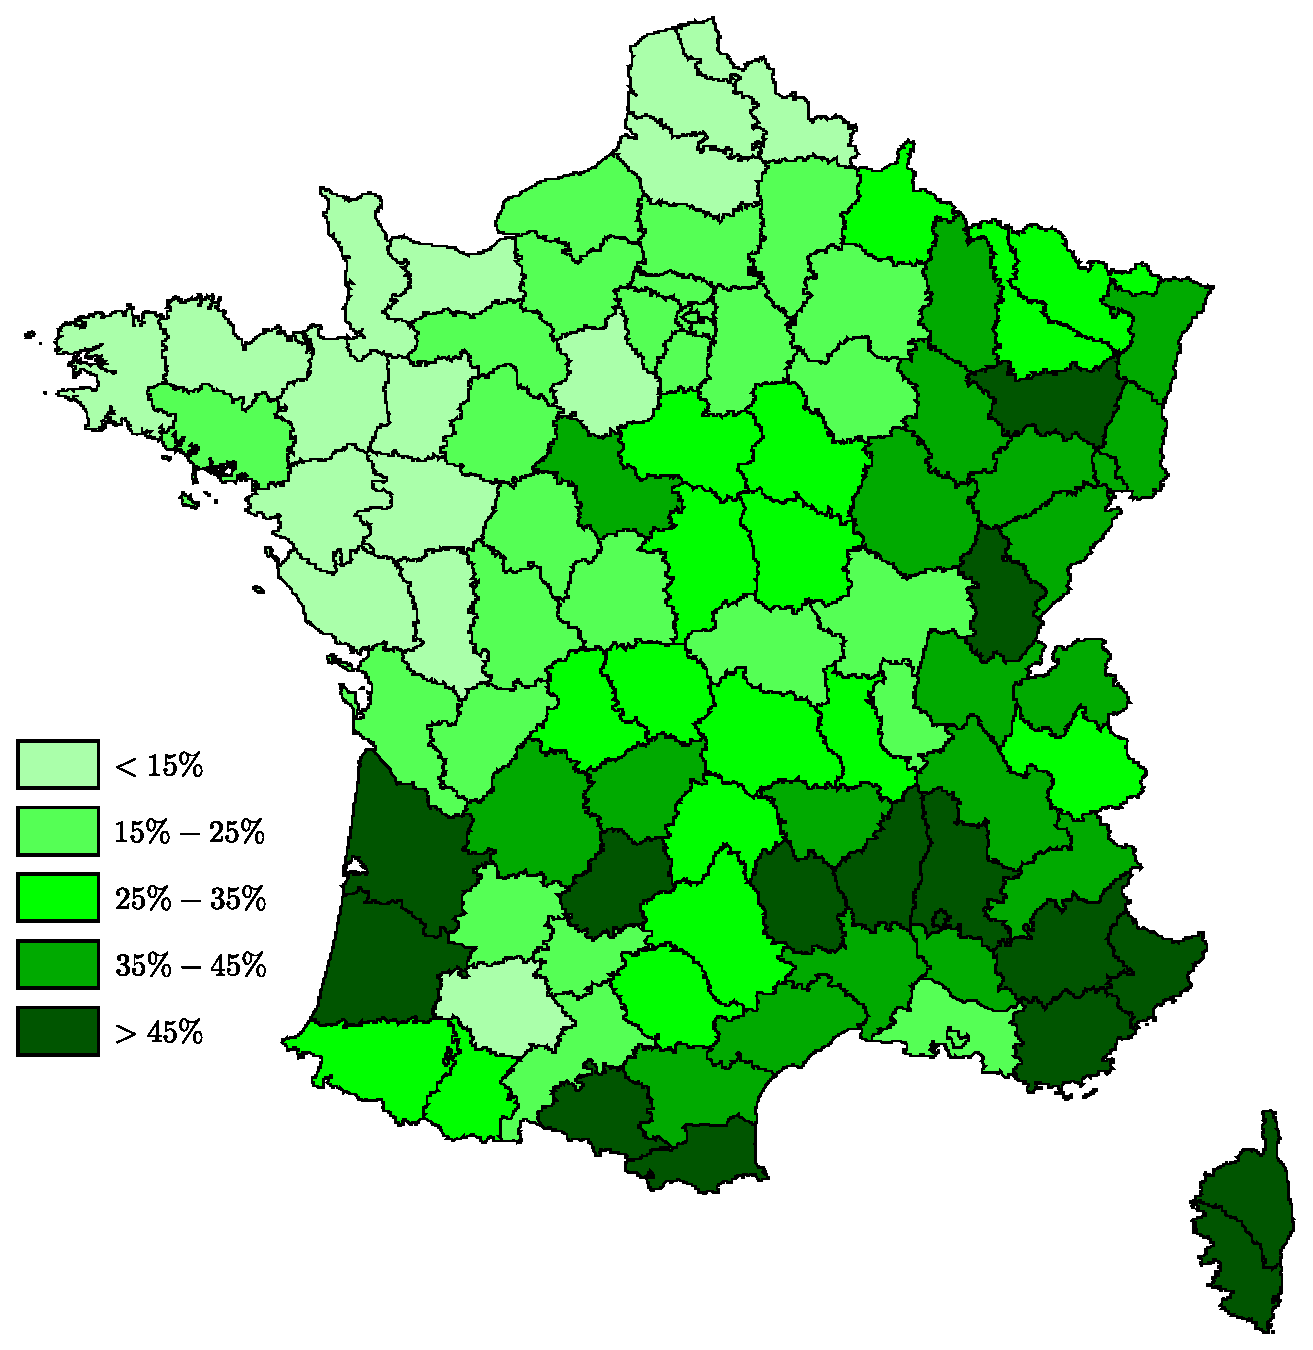
\includegraphics[width=0.8\textwidth]{Figures/boisement}
\end{center}
\caption{Forestation rate in France.}
\label{fig:forestation}
\end{figure}

\begin{figure}[htbp]
\begin{center}
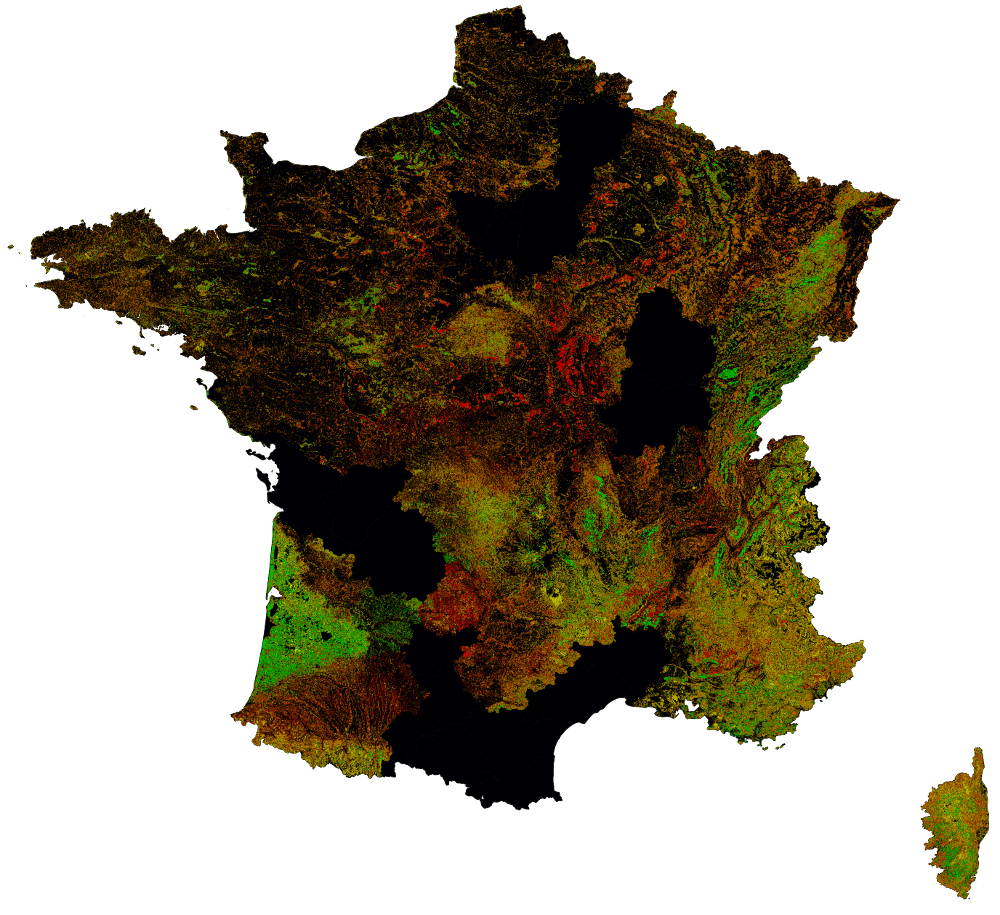
\includegraphics[width=\textwidth]{Figures/BD_foret_France_2}
\end{center}
\caption{The French forest LC. Each color is associated to a single specie ($\sim$20 species in total), black corresponds to non-labeled zones (not operated or non forested).}
\label{fig:FLC}
\end{figure}


\section{Objectives}
Currently, the forest LC is obtained through remote sensing (namely photo-inter\-pretation). A method could be developed to update it automatically. Since an old version of the forest LC is available, it can be used as a ground truth input for subsequent classification \citep{gressin2013updating}. However, the learning process should be carried out carefully \citep{gressin2014updating}. Indeed, some areas might have changed (e.g. forest cuts). Furthermore, the database is designed generalized \citep{smith1977database}. Indeed, forests are not perfectly homogeneous in term of species and there can be many holes in the canopy, leading to a noisy classification. Thus, such classification would then not be sufficient in order to retrieve homogeneous patches similar to the forest LC. In order to retrieve homogeneous patches, the classification could be regularized using smoothing methods \citep{schindler2012overview}. Furthermore, an automatic method considering more data sources than only CIR ortho-images would allow to enrich the LC, i.e. retrieve homogeneous tree species stands also homogeneous in terms of height \citep{gressin2014unified}.

\section{Strategy}
Two remote sensing modalities are available for the mapping of forested areas at IGN; VHR optical images and lidar cloud points. These two modalites are complementary \citep{torabzadeh2014fusion}. Indeed, optical images provide information about the tree species using textural features \citep{franklin2000incorporating}, while the lidar describe the vertical structure, useful for the tree species discrimination \citep{dalponte2012tree, dalponte2014tree}

\paragraph{VHR optical images \\}
The VHR images are a part of a national database. In this thesis, the images used have a spatial resolution of 50$\:$cm. The ortho-images employed have 4 bands (red, green, blue near infra-red) captured by the IGN digital cameras \citep{souchon2012large}. \\
\paragraph{Airborne Laser Scanning \\}
IGN also process lots of flights over forested areas with a laser scanning device. The point density for all echoes ranges from 2 to 4$\:$points/m$^{2}$. \\

The registration between airborne lidar point clouds and VHR multispectral images was performed by IGN itself using ground control points. This is a standard procedure in the French mapping agency since IGN operates both sensors and has also a strong expertise in data georeferencing (this is in fact the national institute responsible for that in France for both airborne and spaceborne sensors). \\

The combination of these two data is very relevant for the study of forest, indeed, optical images provide the major information about the tree species, while lidar give information about the vertical structure of the forest. Furthermore, the lidar allows to extract consistent object such as trees. \\

In order to extract more information from these two modalities, the fusion could be performed at different levels. 3 levels could be defined:
\begin{itemize}
\item[$\bullet$] Low level: It corresponds to the fusion of the observations, in this case, only the reflectance from the optical images and the height of the lidar points.
\item[$\bullet$] Medium level: It corresponds to the fusion of features, derived from both sources, and merged together. It also corresponds to the cooperative understanding of the data; a feature is derived on a modality and applied on the other (e.g. segmentation of the point cloud applied to images).
\item[$\bullet$] High level: It corresponds to decision fusion. One or many classifications have been performed and the final decision is a smart combination of the classifications and the input data.
\end{itemize}

\section{Structure of the thesis}

\begin{itemize}
\item State of the art: Chapter \ref{Chapter1}
\item Method: Chapter \ref{Chapter2}
\item Results: Chapter \ref{Chapter3}
\item Conclusion and perspectives: Chapter \ref{Conclusion}
\end{itemize}

\stopcontents[chapters]
